\section{Contribution of EW Zjj}
\label{sec:miscZstudies}

\graphicspath{{figures/}}

Validation of generator variations produced for Madgraph5 aMC@NLO+pythia8 using Zjj data produced at $\sqrt{s}=8$TeV.

\begin{figure}[h!]
  \centering
  \subfloat[]{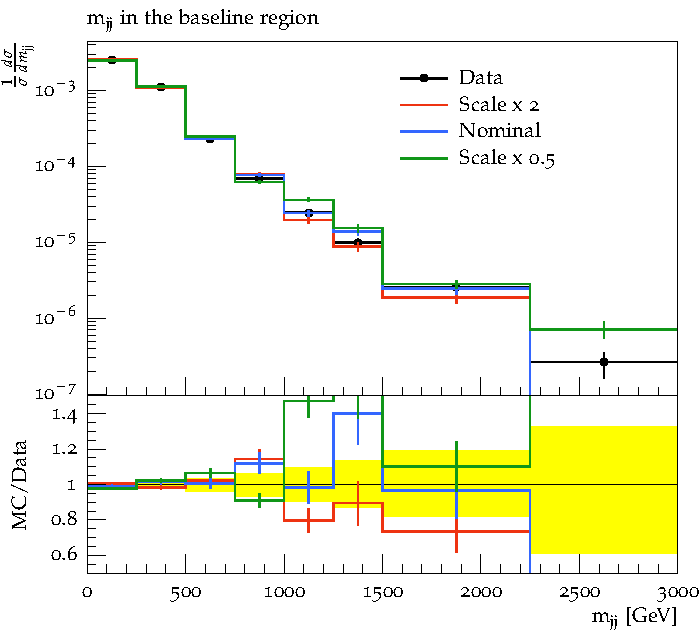
\includegraphics[width=0.45\textwidth]{mjjbase}}
  \subfloat[]{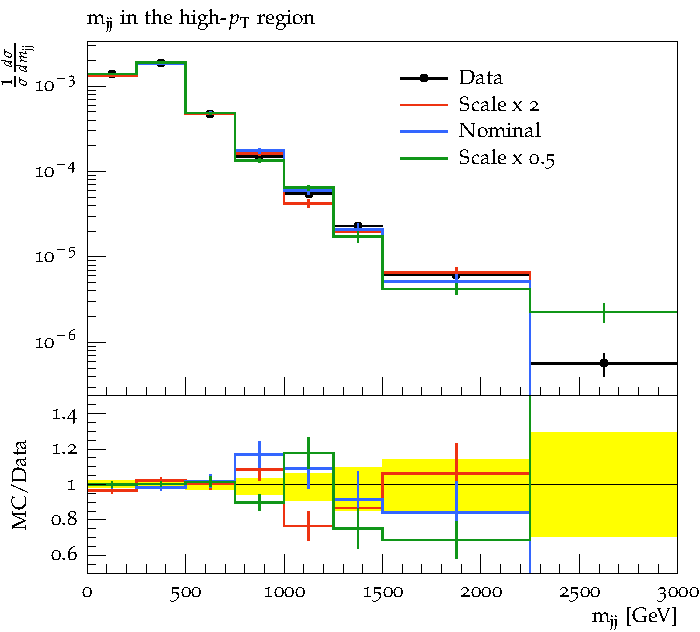
\includegraphics[width=0.45\textwidth]{mjjhighpt}}\\
  \subfloat[]{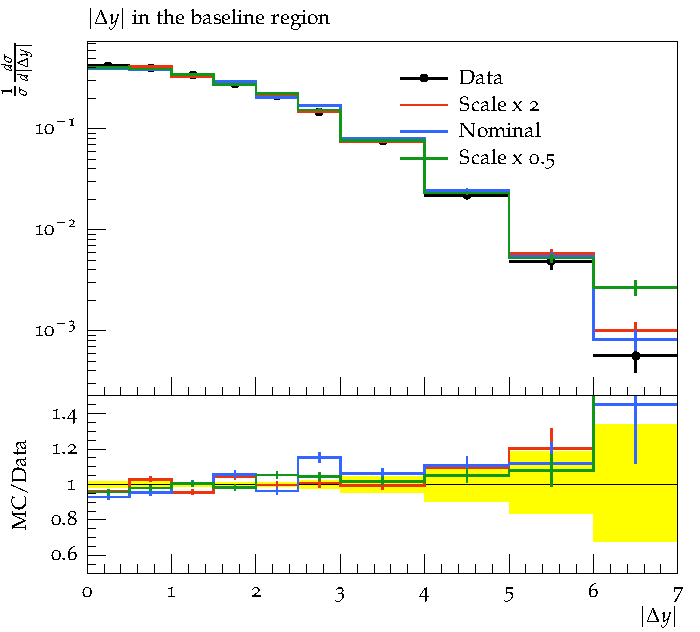
\includegraphics[width=0.45\textwidth]{dybase}}
  \subfloat[]{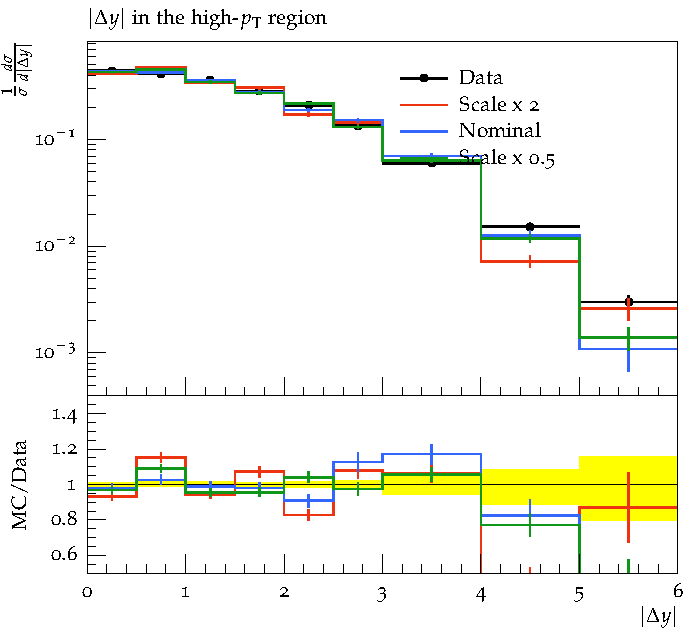
\includegraphics[width=0.45\textwidth]{dyhighpt}}
  \caption{Kinematic distributions of the mass of the dijet system (above) and the difference in rapidity (below) for events with two same flavour leptons in the Z kinematic region. As used for validation of Z MC and for searches for EW production of Zjj at ATLAS}
    \label{fig:Zjj}
\end{figure}

This is run for 2M MC events and normalised to crossection. This is MG5aMC@NLO+pythia8 at 8TeV. This is the process that includes the EW diagrams such that interference is calculated. I'm currently re-running a sample with Strong production and EW production to show effect of interference. Eta 15/07/2016.

If required I can run at 13TeV comparing distributions in our preselection, VBF and Boosted regions with and without EW and with and without interference but no data. Eta 21/07/2016

In progress. 

\section{Effect of Z and Tau polarisations on Z lineshape}
Daniele had vatious suggestions for plots and descriptions here. 